\documentclass{scrartcl}

\usepackage[utf8]{inputenc}
\usepackage[T1]{fontenc}

\usepackage[american]{babel}
\usepackage{listings}
\usepackage{siunitx}
\usepackage{enumitem}
\usepackage{hyperref}
\usepackage{varioref}
\usepackage{amsmath}
\usepackage{pdfpages}

\hypersetup{colorlinks, linkcolor=black}
\KOMAoption{parskip}{half}
\KOMAoption{titlepage}{firstiscover}
\KOMAoption{fontsize}{11pt}
\setlist[description]{noitemsep,font=\ttfamily}

\newcommand{\amf}{a_\mathrm{mf}}
\newcommand{\bxv}{b_\mathrm{xv}}

\begin{document}

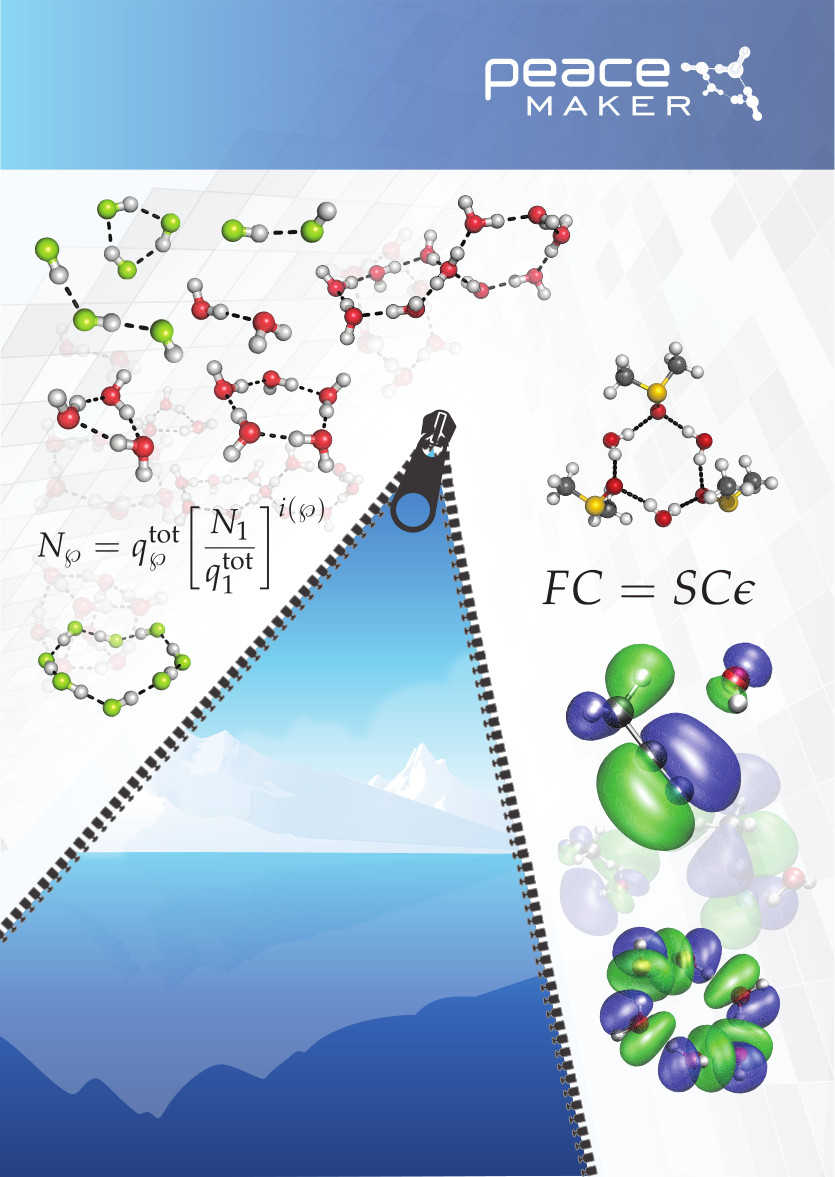
\includepdf[pages={1}]{cover.jpg}

\title{Peacemaker Manual}
\author{Michael von Domaros}
\begin{titlepage}
    \centering
    \Large

    \vspace*{5ex}
    \textbf{\Huge Peacemaker Manual}

    \vspace{\fill}
    written by
    
    \vspace{1ex}
    Michael von Domaros,\\
    Johannes Ingenmey
    
    \vspace{2ex}
    \today
    \vspace{\fill}
\end{titlepage}

\tableofcontents
\pagebreak


\section{Compiling Peacemaker}

Peacemaker is a modern FORTRAN code and thus requires a modern FORTRAN compiler.
We recommend a recent version of gfortran which is used for active development.

Peacemaker can be built by running
\begin{addmargin}[1cm]{0cm}
    \ttfamily
    \$ make release
\end{addmargin}
which should produce a run time optimized binary called peacemaker.
In case of errors, adjust the makefile to your compiler.
We recommend the following compiler flags or your compiler's equivalents:
\begin{addmargin}[1cm]{0cm}
    \begin{description}
        \item[-O3] highest optimization level that guarantees standard compliance
        \item[-fopenmp] OpenMP parallelization
        \item[-flto] link-time optimization
    \end{description}
\end{addmargin}

A version suitable for development and debugging can be built by running
\begin{addmargin}[1cm]{0cm}
    \ttfamily
    \$ make debug
\end{addmargin}

Note: Older versions of gfortran are subject to a bug which prevents OpenMP parallelization.
If you receive the error message ``Attempting to allocate already allocated variable `ib' '', compile without OpenMP support, or upgrade to a newer compiler version.

\section{Running Peacemaker}

Peacemaker is run by
\begin{addmargin}[1cm]{0cm}
    \ttfamily
    \$ peacemaker [input] [clusterset]
\end{addmargin}
where \texttt{[input]} is the location of the input file and \texttt{[clusterset]} is the location of the clusterset file.
The structure of both files will be explained in section \vref{sec:config}.

If Peacemaker was compiled with OpenMP parallelization, it can be run in parallel by
\begin{addmargin}[1cm]{0cm}
    \ttfamily
    \$ OMP\_NUM\_THREADS=[N] peacemaker [input] [clusterset]
\end{addmargin}
In this case, \texttt{[N]} specifies the number of threads to run with.

\section{Parallelization Strategy}

Peacemaker parallelizes the $\amf$, $\bxv$ sampling.
The workload is shared among all available threads.
Thus almost perfect parallel efficiency can be expected for large sampling ranges (or a fine grid), but no speedup should be expected
if a very large number of clusters or many temperatures are investigated.

\section{Peacemaker Configuration Files}
\label{sec:config}

Both the input and the clusterset file share a common format which shall be briefly explained here.
The general structure of any of those files is:

\begin{addmargin}[1cm]{0cm}
    \ttfamily
    \begin{minipage}{\textwidth}
        [section1]
        \begin{addmargin}[1cm]{0cm}
            keyword1 argument1 argument2 ...\#\ comment \\
            keyword2 argument1 argument2 ...\\
            ...
        \end{addmargin}
    \end{minipage}

    \begin{minipage}{\textwidth}
        [section2]
        \begin{addmargin}[1cm]{0cm}
            keyword1 argument1 argument2 ... \\
            keyword2 argument1 argument2 ... \\
            ...
        \end{addmargin}
    \end{minipage}

    \begin{minipage}{\textwidth}
        ...
    \end{minipage}

\end{addmargin}

Thus there are sections, which shall be embraced in brackets, keywords, arguments, and comments.
Section labels are unique.
Keywords within a section are unique.
Arguments are optional.
Comments may start anywhere and are introduced by the number sign \#.
All elements are case sensitive.

\section{The Peacemaker Input File}
\label{sec:input}

\subsection{Examples}

The following input file will run a QCE "single point" calculation for a one-component system using the clusterset specified in the command line and explained in section~\vref{sec:clusterset}.
Default options are used in most cases.

\begin{addmargin}[1cm]{0cm}
    \ttfamily
    \begin{minipage}{\textwidth}
        [qce]
        \begin{addmargin}[1cm]{0cm}
            amf 0.1 \# J*m\^{}3/mol\^{}2 \\
            bxv 1.3
        \end{addmargin}
    \end{minipage}

    \begin{minipage}{\textwidth}
        [ensemble]
        \begin{addmargin}[1cm]{0cm}
            temperature 200.0 400.0 201 \# K \\
            pressure 1.01325 \# bar \\
            monomer\_amounts 1.0 \# mol
        \end{addmargin}
    \end{minipage}
\end{addmargin}

The following input will perform an $\amf$, $\bxv$ parameter sampling for a pure substance.
Reference data are provided by an isobar file.
Further details on parameter sampling are explained in section~\vref{sec:sampling}.

\begin{addmargin}[1cm]{0cm}
    \ttfamily
    \begin{minipage}{\textwidth}
        [system]
        \begin{addmargin}[1cm]{0cm}
            components 1
        \end{addmargin}
    \end{minipage}

    \begin{minipage}{\textwidth}
        [qce]
        \begin{addmargin}[1cm]{0cm}
            amf 0.0 0.5 101 \# J*m\^{}3/mol\^{}2 \\
            bxv 1.0 2.0 101
        \end{addmargin}
    \end{minipage}

    \begin{minipage}{\textwidth}
        [ensemble]
        \begin{addmargin}[1cm]{0cm}
            temperature 200.0 400.0 201 \# K \\
            pressure 1.01325 \# bar \\
            monomer\_amounts 1.0 \# mol
        \end{addmargin}
    \end{minipage}

    \begin{minipage}{\textwidth}
        [reference]
        \begin{addmargin}[1cm]{0cm}
            isobar isobar.dat
        \end{addmargin}
    \end{minipage}
\end{addmargin}

The following input will perform an $\amf^{\mathrm{mix}}$ parameter sampling for a binary mixture.
Reference data are provided by a density at \SI{298.15}{K} and a temperature of phase transition.

\begin{addmargin}[1cm]{0cm}
    \ttfamily
    \begin{minipage}{\textwidth}
        [system]
        \begin{addmargin}[1cm]{0cm}
            components 2
        \end{addmargin}
    \end{minipage}

    \begin{minipage}{\textwidth}
        [qce]
        \begin{addmargin}[1cm]{0cm}
            bxv\_pure 1.2 1.6 \\
            amf\_pure 0.2 0.8 \# J*m\^{}3/mol\^{}2 \\
            amf\_mix 0.0 0.5 101 \# J*m\^{}3/mol\^{}2
        \end{addmargin}
    \end{minipage}

    \begin{minipage}{\textwidth}
        [ensemble]
        \begin{addmargin}[1cm]{0cm}
            temperature 200.0 400.0 201 \# K \\
            pressure 1.01325 \# bar \\
            monomer\_amounts 0.5 0.5 \# mol
        \end{addmargin}
    \end{minipage}

    \begin{minipage}{\textwidth}
        [reference]
        \begin{addmargin}[1cm]{0cm}
            density 298.15 1.023 \# K; g/cm\^{}3 \\
            phase\_transition 373.15 \# K
        \end{addmargin}
    \end{minipage}
\end{addmargin}

The following input will perform an $\amf$, $\bxv$ parameter optimization for a ternary mixture, following a rough sampling on a small grid.
Reference data are provided by a density at \SI{298.15}{K} and a temperature of phase transition.

\begin{addmargin}[1cm]{0cm}
    \ttfamily
    \begin{minipage}{\textwidth}
        [system]
        \begin{addmargin}[1cm]{0cm}
            components 3
        \end{addmargin}
    \end{minipage}

    \begin{minipage}{\textwidth}
        [qce]
        \begin{addmargin}[1cm]{0cm}
            amf 0.0 2.0 11 \# J*m\^{}3/mol\^{}2 \\
            bxv 0.5 1.5 11 \\
            grid\_iterations 2 \\
            optimizer 1
        \end{addmargin}
    \end{minipage}

    \begin{minipage}{\textwidth}
        [ensemble]
        \begin{addmargin}[1cm]{0cm}
            temperature 273.15 400.15 128 \# K \\
            pressure 1.01325 \# bar \\
            monomer\_amounts 0.6 0.1 0.3 \# mol
        \end{addmargin}
    \end{minipage}

    \begin{minipage}{\textwidth}
        [reference]
        \begin{addmargin}[1cm]{0cm}
            density 298.15 0.9248 \# K; g/cm\^{}3 \\
            phase\_transition 332.61 \# K
        \end{addmargin}
    \end{minipage}
\end{addmargin}

While hopefully self-explaining, all sections and their associated keywords shall be explained in the following.

\subsection{Section [system]}

\begin{description}
    \item[components N] \hfill \\
        The number of components in the system.
        Currently only 1 (pure) and 2 (binary) are supported.
        Note that although it is possible to run a pure system as binary system, where the amount of one of the species is set to zero, we strongly encourage you to run such calculations as a pure system.
        Results will be the same in either case, but slow convergence may arise for some temperatures if the amount of monomers of one component is sufficiently small.
        Optional. Default: 1
\end{description}

\subsection{Section [qce]}

\begin{description}
    \item[amf A]
    \item[amf A B N] \hfill \\
        The mean field parameter $\amf$ in units of \si{\joule\cubic\meter\per\mole\squared}.
        Can be specified either as a single value A, or as a range A, B, N, where A is the start, B the end, and N the number of data points (including both boundaries).
        For multi-component mixtures, this keyword is equivalent to \texttt{amf\_mix}.
        Optional. Default: 0.0
        \vspace{0.1cm}
    \item[amf\_pure A B C ...] \hfill \\
        The pure-component mean field parameters $\amf^{a}$, $\amf^{b}$, ..., $\amf^{n}$ in units of \si{\joule\cubic\meter\per\mole\squared}.
        May be specified for multi-component mixtures only.
        Optional. If unspecified, $\amf^a = \amf^b = ... = \amf^n = \amf^{ab...n}$ is used.
        \vspace{0.1cm}
    \item[amf\_mix A]
    \item[amf\_mix A B N] \hfill \\
        The mixed-species mean field parameter $\amf^{ab}$ in units of \si{\joule\cubic\meter\per\mole\squared}.
        Can be specified either as a single value A, or as a range A, B, N, where A is the start, B the end, and N the number of data points (including both boundaries).
        For multi-component mixtures, this keyword is equivalent to \texttt{amf}.
        Optional. Default: 0.0
        \vspace{0.1cm}
    \item[bxv A]
    \item[bxv A B N] \hfill \\
        The exclusion volume scaling parameter $\bxv$.
        Can be specified either as a single value A, or as a range A, B, N, where A is the start, B the end, and N the number of data points (including both boundaries).
        Optional. Default: 1.0
        \vspace{0.1cm}
    \item[bxv\_pure A B] \hfill \\
        The pure-component exclusion volume scaling parameters $\bxv^{a}$ and $\bxv^{b}$.
        May be specified for binary mixtures only.
        Optional. Default: 1.0
        \vspace{0.1cm}
    \item[grid\_iterations A] \hfill \\
        The number of iterations for the parameter sampling if a sampling grid is specified.
        With each iteration, the grid center is moved to the best parameter pair and the grid size is decreased with a factor of 0.2.
        Optional. Default: 1
    \item[optimizer A] \hfill \\
        Specifies which optimization algorithm will be used.
        Can be set to 0 (no optimization) or 1 (Nelder-Mead method).
        Optional. Default: 0
    \item[rotor\_cutoff A] \hfill \\
        The cutoff frequency in cm$^{-1}$ at which the RRHO-correction for low frequencies will be used.
        To limit their influence on the entropy, vibrational modes with a frequency below A will be treated as hindered rotations, employing a switching function to smooth the transition between harmonic oscillator and rigid rotator. If set to 0, no correction will be applied.
        Optional. Default: 0
    \item[max\_deviation A] \hfill \\
        The maximum relative deviation of the Gibbs energy.
        Used to check convergence of the QCE iteration.
        A QCE cycle has converged, if \[\left|\frac{G(\text{current step}) - G(\text{last step})}{G(\text{last step})}\right| < A.\]
        Optional. Default: 1.0e-9
        \vspace{0.1cm}
    \item[volume\_damping\_factor A] \hfill \\
        The volume damping factor used to damp the initial volume guess if one of the polynomials did not converge.
        Shall be between 0 and 1.
        Damping is performed by $\gamma_V = 1 \pm A$, depending on the mode of the temperature loop.
        Optional. Default: 0.01
        \vspace{0.1cm}
    \item[qce\_iterations N] \hfill \\
        The maximum number of iterations in a QCE cycle.
        Optional. Default: 100
        \vspace{0.1cm}
    \item[newton\_iterations N] \hfill \\
        The maximum number of iterations in a Newton--Raphson cycle.
        Optional. Default: 500
\end{description}

\subsection{Section [reference]}

This section is optional.
It enables comparison to experimental reference data.
It is disabled by default.
Further details on parameter sampling are given in section~\vref{sec:sampling}.

\begin{description}
    \item[density A B]
    \item[density A B C] \hfill \\
        Reference density B in units of \si{\gram\per\cubic\centi\meter} at reference temperature A in \si{\kelvin} and an optional error weight C.
        Optional.
        \vspace{0.1cm}
    \item[isobar P]
    \item[isobar P A] \hfill \\
        Path to an isobar file P and an optional error weight A.
        Isobar files contain two columns representing the temperature in \si{\kelvin} and volume in \si{\liter}.
        Optional.
        \vspace{0.1cm}
    \item[phase\_transition A]
    \item[phase\_transition A B] \hfill \\
        Reference temperature of phase transition A in units of \si{\kelvin} and an optional error weight B.
        Optional.
\end{description}

\subsection{Section [output]}

This section is optional.
It enables output control.
It is disabled by default.

\begin{description}
    \item[contributions]
    \item[contributions <helmholtz|internal|entropy|cv>] \hfill \\
        Enables the output of contributions of each degree of freedom to the thermodynamic functions.
        If no arguments are given, contribution output is enabled for all possible thermodynamic quantities.
        If arguments are specified, contribution output is only enabled for the selected thermodynamic quantities.
        Optional.
    \item[progress]
    \item[noprogress] \hfill \\
        Enables or disables the progress bar.
        Optional. Default: enabled.
\end{description}

\section{The Peacemaker Clusterset File}
\label{sec:clusterset}

\subsection{Example}

Clusterset files are structured like input files.
A section provides all necessary information about a cluster.
The section label is used as cluster label.
Cluster data may be acquired with the help of the tools provided with this distribution of Peacemaker.
See the tools/README file for further information.

\clearpage
\begin{addmargin}[1cm]{0cm}
    \ttfamily
    [Cluster 1]
    \begin{addmargin}[1cm]{0cm}
        monomer \\
        composition 1 \\
        sigma 2 \\
        coordinates /home/user/clusters/cluster1.xyz \\
        frequencies /home/user/clusters/cluster1.flist \\
        energy 0.0 \\
        volume 60.0 \\
        frequency\_scale 0.97
    \end{addmargin}
    [Cluster 2]
    \begin{addmargin}[1cm]{0cm}
        composition 3 \\
        sigma 3 \\
        coordinates /home/user/clusters/cluster2.xyz \\
        frequencies /home/user/clusters/cluster2.flist \\
        energy -20.0 \\
        frequency\_scale 0.97
    \end{addmargin}
    ...
\end{addmargin}

\subsection{Details}

\begin{description}
    \item[monomer] \hfill \\
        Sets the current cluster as monomer.
        Optional, but must be present once for each component.
        \vspace{0.1cm}
    \item[composition N M] \hfill \\
        Composition of the cluster in number of monomers.
        One number for each component.
        \vspace{0.1cm}
    \item[sigma N] \hfill \\
        The rotational symmetry number of the cluster.
        \vspace{0.1cm}
    \item[coordinates P] \hfill \\
        Path to a coordinate file in the xyz format.
        Units are \si{\angstrom}.
        \vspace{0.1cm}
    \item[frequencies P] \hfill \\
        Path to a frequency file.
        It contains the number of frequencies in line 1, followed by a comment line, followed by one frequency per line.
        Units are \si{\per\centi\meter}.
        \vspace{0.1cm}
    \item[energy A] \hfill \\
        The adiabatic interaction energy of the cluster in units of \si{\kilo\joule\per\mol} (negative energies represent stable clusters).
        \vspace{0.1cm}
    \item[volume A] \hfill \\
        The volume of the cluster in units of \si{\cubic\angstrom}.
        Must be specified for monomers, only.
        \vspace{0.1cm}
    \item[frequency\_scale A] \hfill \\
        A frequency scaling factor.
        Optional.
        \vspace{0.1cm}
    \item[anharmonicity A] \hfill \\
        The anharmonicity constant.
        Optional.
\end{description}

\section{Peacemaker Output Files}

Peacemaker writes results for the best $\amf$, $\bxv$ parameter pair if it could be determined or for the first $\amf$, $\bxv$ pair otherwise.
In the following, the output files shall be briefly described.
All output files contain the temperature in \si{K} in column 1.

\begin{description}
    \item[volume.dat] \hfill \\
        Contains the volume and related quantities:
        volume $V$ in \si{dm^3}, exclusion volume $V_\mathrm{excl}$ in \si{dm^3}, volumetric expansion coefficient $\alpha$ in $\si{K^{-1}}$, status code for debugging purposes.
        \vspace{0.1cm}
    \item[thermo0.dat] \hfill \\
        Contains thermodynamic quantities that do not depend on any derivative:
        Helmholtz free energy $A$ in \si{kJ}, Gibbs free energy $G$ in \si{kJ}.
        \vspace{0.1cm}
    \item[thermo1.dat] \hfill \\
        Contains thermodynamic quantities that depend on first derivatives:
        internal energy $U$ in \si{kJ}, enthalpy $H$ in \si{kJ}, entropy $S$ in \si{J/K}.
        \vspace{0.1cm}
    \item[thermo2.dat] \hfill \\
        Contains thermodynamic quantities that depend on second derivatives:
        heat capacity at constant volume $c_V$ in \si{J/K}, heat capacity at constant pressure $c_P$ in \si{J/K}.
        \vspace{0.1cm}
    \item[xxx\_contrib.dat] \hfill \\
        Contains contributions of each degree of freedom to the quantity denoted by xxx.
        Possible quantities are: Helmholtz free energy, internal energy, entropy, heat capacity at constant volume.
        \vspace{0.1cm}
    \item[xxx\_clusters.dat] \hfill \\
        Contains the contributions of each cluster to the quantity denoted by xxx divided by its absolute population (meaning these are cluster specific quantities).
        Possible quantities are: the partition function and its derivatives, the indistinguishability contribution, Helmholtz free energy, internal energy, Gibbs energy, enthalpy entropy, heat capacity at constant volume and pressure.
        \vspace{0.1cm}
    \item[populations.dat] \hfill \\
        Contains populations of each cluster in the order they were specified in the clusterset.
        Populations are monomer normalized.
        For example, in a binary system:
        \begin{align}
        N^\prime_\wp = \frac{\left(i_\wp+j_\wp\right)N_\wp}{N_\text{1,tot} + N_\text{2,tot}}.
        \end{align}
        Generally, in a multi-component system:
        \begin{align}
        \qquad N^\prime_\wp = \sum_\mathrm{c} \frac{i_\mathrm{c} \cdot N_\wp}{N_\mathrm{c,tot}}.
        \end{align}
        \vspace{0.1cm}
    \item[concentrations.dat] \hfill \\
        Contains concentrations in $\si{mol/l}$ of each cluster in the order they were specified in the clusterset.
        Concentrations are not monomer normalized.
\end{description}

\section{Parameter Sampling}
\label{sec:sampling}

Peacemaker performs $\amf$, $\bxv$ parameter sampling on a grid, which can be specified in the [qce] section of the input file.
For each pair, the quality of the resulting isobar is compared to certain experimental quantities.
The following options are available for this purpose: single density, isobar, temperature of phase transition.
The isobar quality is computed according to the following equation.
\begin{equation*}
    \mathrm{error} = w_\mathrm{density}                                      {\left(\frac{\rho - \rho^\mathrm{exp}}{\rho^\mathrm{exp}}\right)}^2
                   + w_\mathrm{isobar}            \frac{1}{N} \sum_{i=1}^{N} {\left(\frac{V_i - V_i^\mathrm{exp}}{V_i^\mathrm{exp}}\right)}^2
                   + w_\mathrm{phase\ transition}                            {\left(\frac{T_\mathrm{pt}-T_\mathrm{pt}^\mathrm{exp}}{T_\mathrm{pt}^\mathrm{exp}}\right)}^2
\end{equation*}
Any combination of the experimental data above can be chosen.
The relative importance of each quantity can be specified by the weight $w$.

Isobars are specified by an isobar file.
This file shall contain two columns of numbers: temperatures in \si{K} in column one and volumes in \si{\cubic\deci\meter} in column two.
All temperatures must be within the temperature range specified in the [qce] section.
There are no requirements on the order of the temperatures.
Temperatures may be included multiple times to put special weight on them.
If a reference temperature is not equal to the temperature specified by the temperature range in the [qce] section, linear interpolation between the two closest temperatures is performed.

\end{document}
